\pdfminorversion=4
\documentclass[aspectratio=169]{beamer}

\mode<presentation>
{
  \usetheme{default}
  \usecolortheme{default}
  \usefonttheme{default}
  \setbeamertemplate{navigation symbols}{}
  \setbeamertemplate{caption}[numbered]
  \setbeamertemplate{footline}[frame number]  % or "page number"
  \setbeamercolor{frametitle}{fg=white}
  \setbeamercolor{footline}{fg=black}
} 

\usepackage[english]{babel}
\usepackage{inputenc}
\usepackage{tikz}
\usepackage{courier}
\usepackage{array}
\usepackage{bold-extra}
\usepackage{minted}
\usepackage[thicklines]{cancel}
\usepackage{fancyvrb}

\xdefinecolor{dianablue}{rgb}{0.18,0.24,0.31}
\xdefinecolor{darkblue}{rgb}{0.1,0.1,0.7}
\xdefinecolor{darkgreen}{rgb}{0,0.5,0}
\xdefinecolor{darkgrey}{rgb}{0.35,0.35,0.35}
\xdefinecolor{darkorange}{rgb}{0.8,0.5,0}
\xdefinecolor{darkred}{rgb}{0.7,0,0}
\definecolor{darkgreen}{rgb}{0,0.6,0}
\definecolor{mauve}{rgb}{0.58,0,0.82}

\title[2024-10-20-preCHEP-2024-codas-hep]{CoDaS-HEP, US-CMS, US-ATLAS}
\author{Jim Pivarski}
\institute{Princeton University -- IRIS-HEP}
\date{October 10, 2024}

\usetikzlibrary{shapes.callouts}

\begin{document}

\logo{\pgfputat{\pgfxy(0.11, 7.4)}{\pgfbox[right,base]{\tikz{\filldraw[fill=dianablue, draw=none] (0 cm, 0 cm) rectangle (50 cm, 1 cm);}\mbox{\hspace{-8 cm}
\includegraphics[height=1 cm]{princeton-logo-long.png}\hspace{0.1 cm}\raisebox{0.1 cm}{
\includegraphics[height=0.8 cm]{iris-hep-logo-long.png}}\hspace{0.1 cm}}}}}

\begin{frame}
  \titlepage
\end{frame}

\logo{\pgfputat{\pgfxy(0.11, 7.4)}{\pgfbox[right,base]{\tikz{\filldraw[fill=dianablue, draw=none] (0 cm, 0 cm) rectangle (50 cm, 1 cm);}\mbox{\hspace{-8 cm}
\includegraphics[height=1 cm]{princeton-logo.png}\hspace{0.1 cm}\raisebox{0.1 cm}{
\includegraphics[height=0.8 cm]{iris-hep-logo.png}}\hspace{0.1 cm}}}}}

% Uncomment these lines for an automatically generated outline.
%\begin{frame}{Outline}
%  \tableofcontents
%\end{frame}

% START START START START START START START START START START START START START

\begin{frame}{Three of this year's HEP-computing tutorials in the U.S.}
\Large
\vspace{0.5 cm}
\begin{columns}
\column{1.08\linewidth}
\begin{itemize}\setlength{\itemsep}{0.5 cm}
\item June 20--21 (2 days): US-CMS at Princeton

\textcolor{gray}{\normalsize Alexander Held, Andrzej Novak, Elliott Kauffman, Jim Pivarski, Lindsey Gray, \\ Matthew Feickert, Nick Manganelli, Nick Smith, Oksana Shadura, Peter Elmer}

\item July 18--19 (2 days): US-ATLAS at U.\ Washington

\textcolor{gray}{\normalsize Alexander Held, Ana Peixoto, Fengping Hu, Gordon Watts, Jim Pivarski, \\ Kyungeon Choi, Lindsey Gray, Matthew Feickert, Oksana Shadura, Vangelis Kourlitis}

\item July 22--26 (5 days): CoDaS-HEP at Princeton

\textcolor{gray}{\normalsize Andres Rios-Tascon, David Lange, Henry Schreiner, Ianna Osborne, Jim Pivarski, Kilian Lieret, Louis-Guillaume Gagnon, Peter Elmer, Steve Lantz, Sudhir Malik, Tim Mattson}
\end{itemize}
\end{columns}
\end{frame}

\begin{frame}{Photos (from CoDaS-HEP)}
\vspace{0.5 cm}
\begin{columns}
\column{0.33\linewidth}
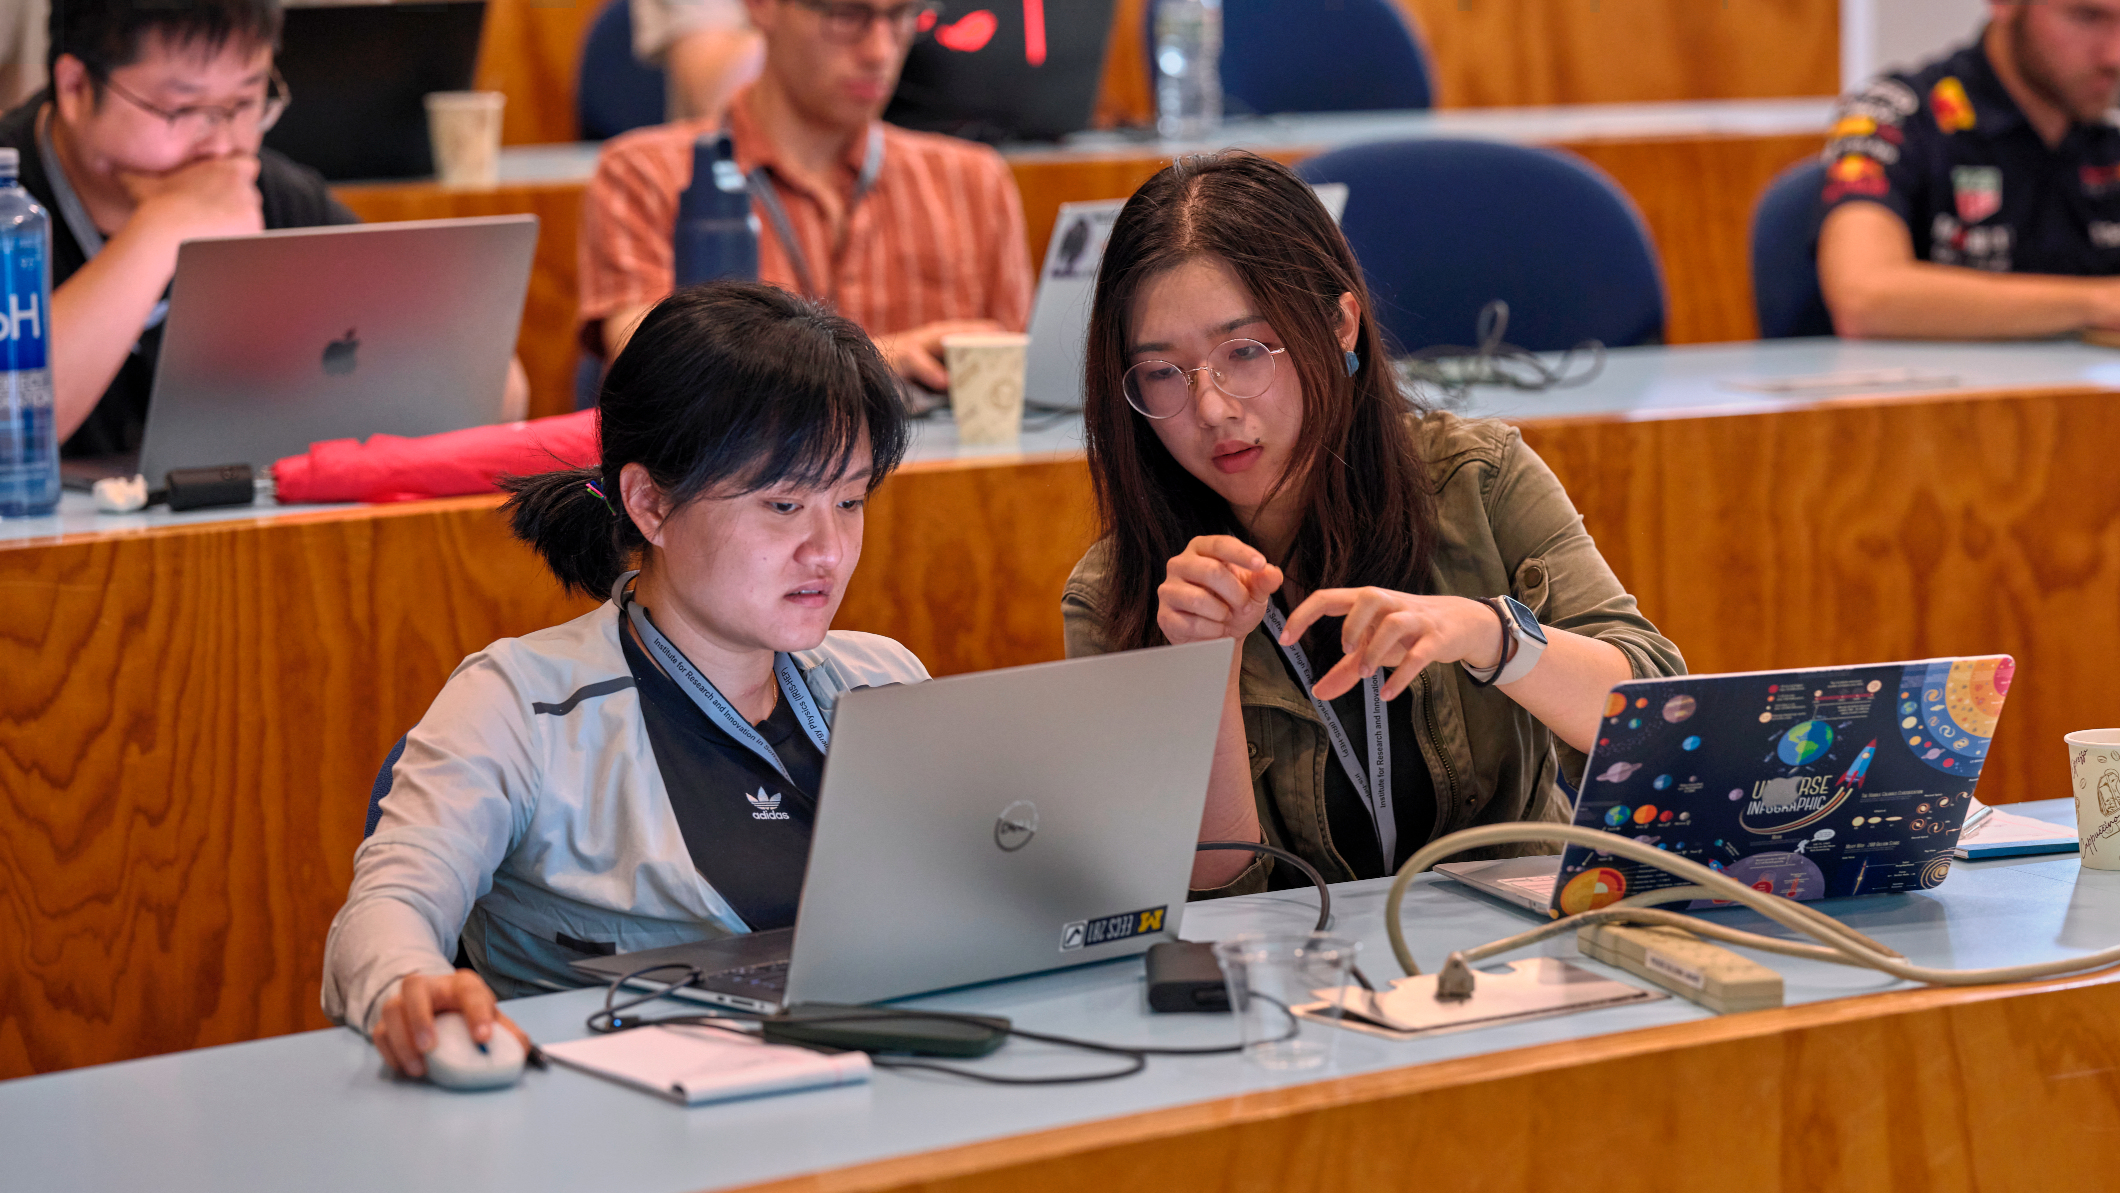
\includegraphics[width=\linewidth]{PHOTOS/DSCF2628.jpg}

\column{0.33\linewidth}
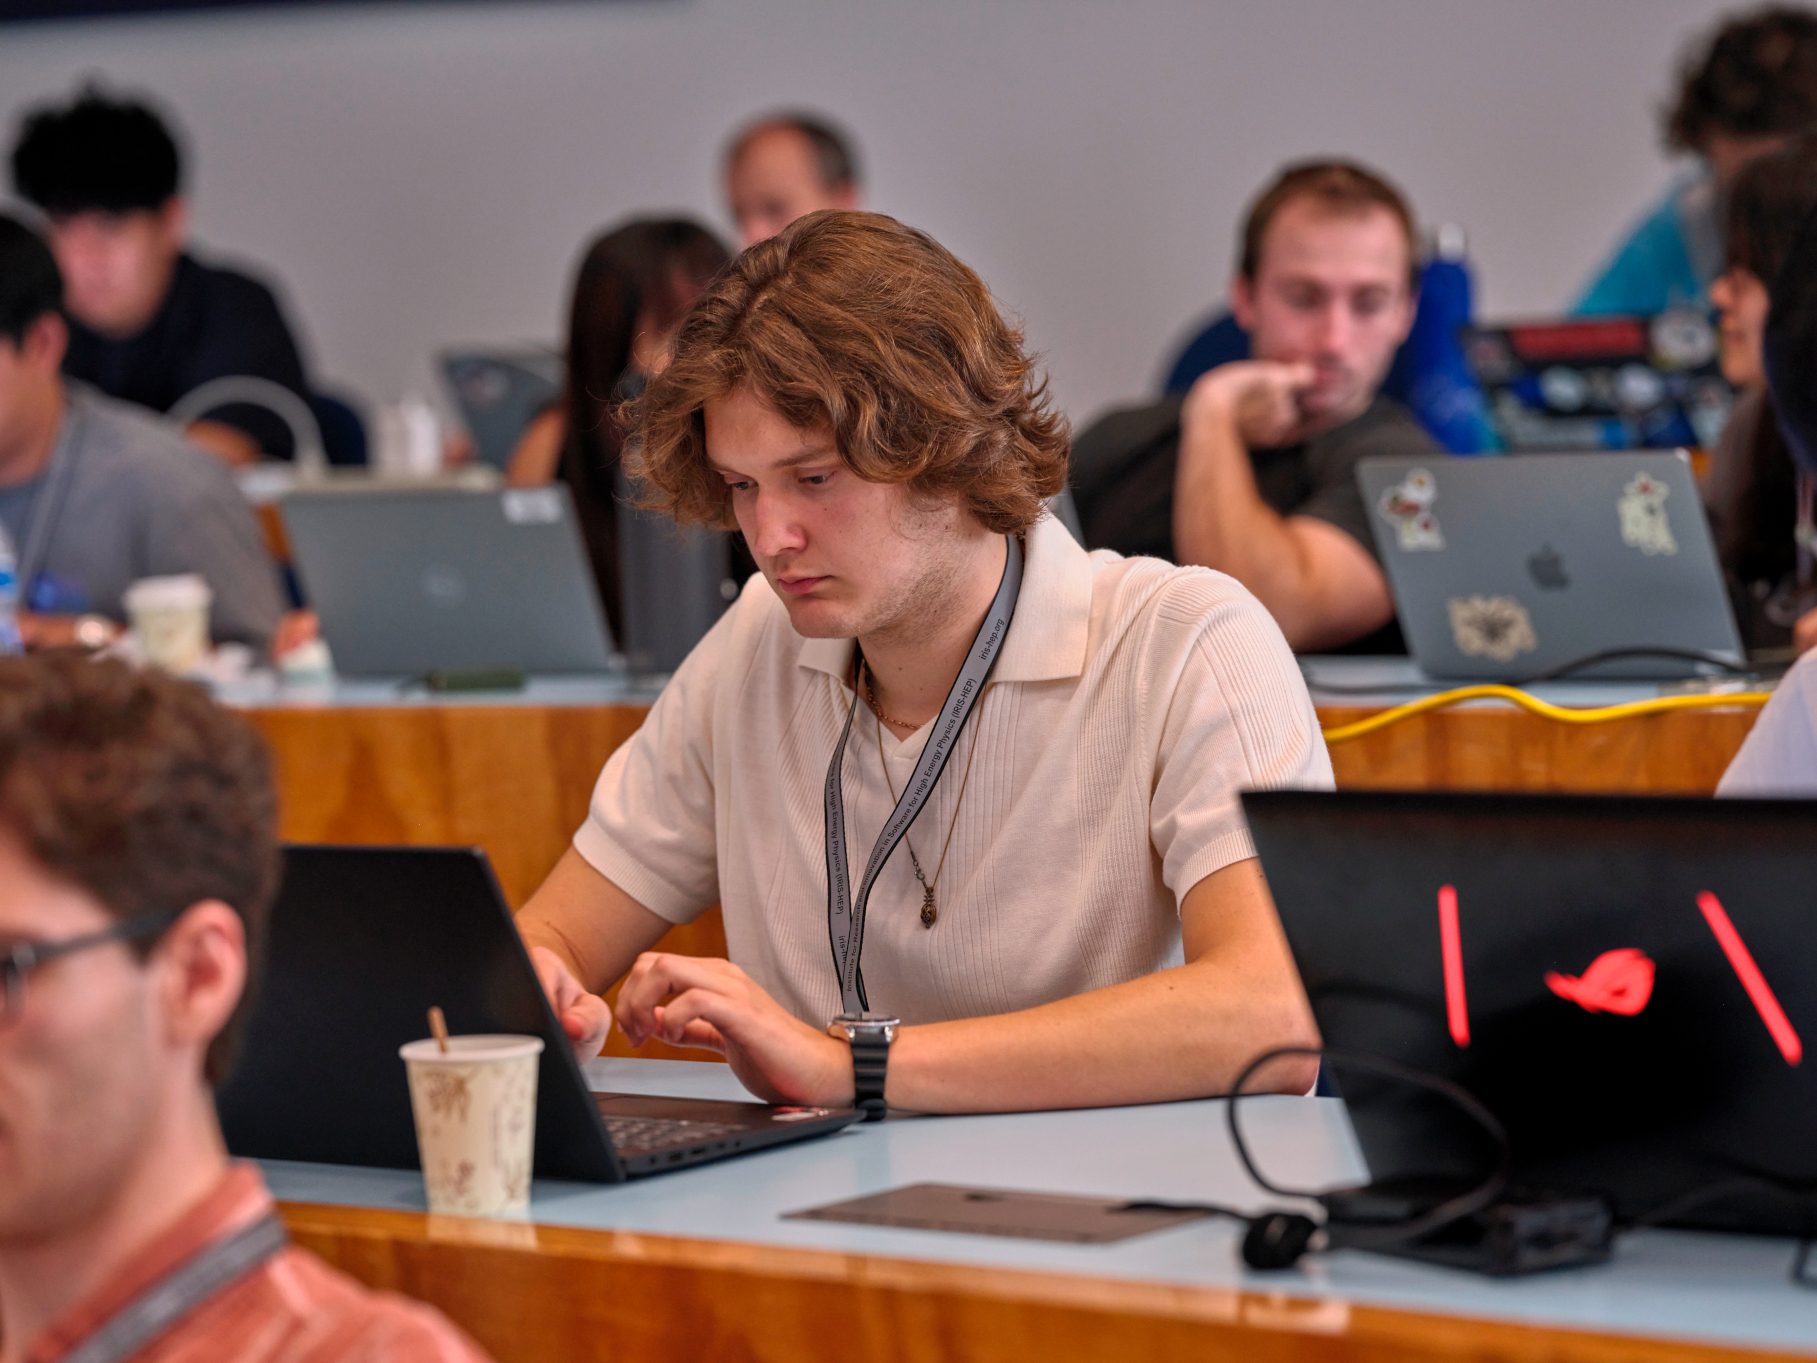
\includegraphics[width=\linewidth]{PHOTOS/DSCF2637.jpg}

\column{0.33\linewidth}
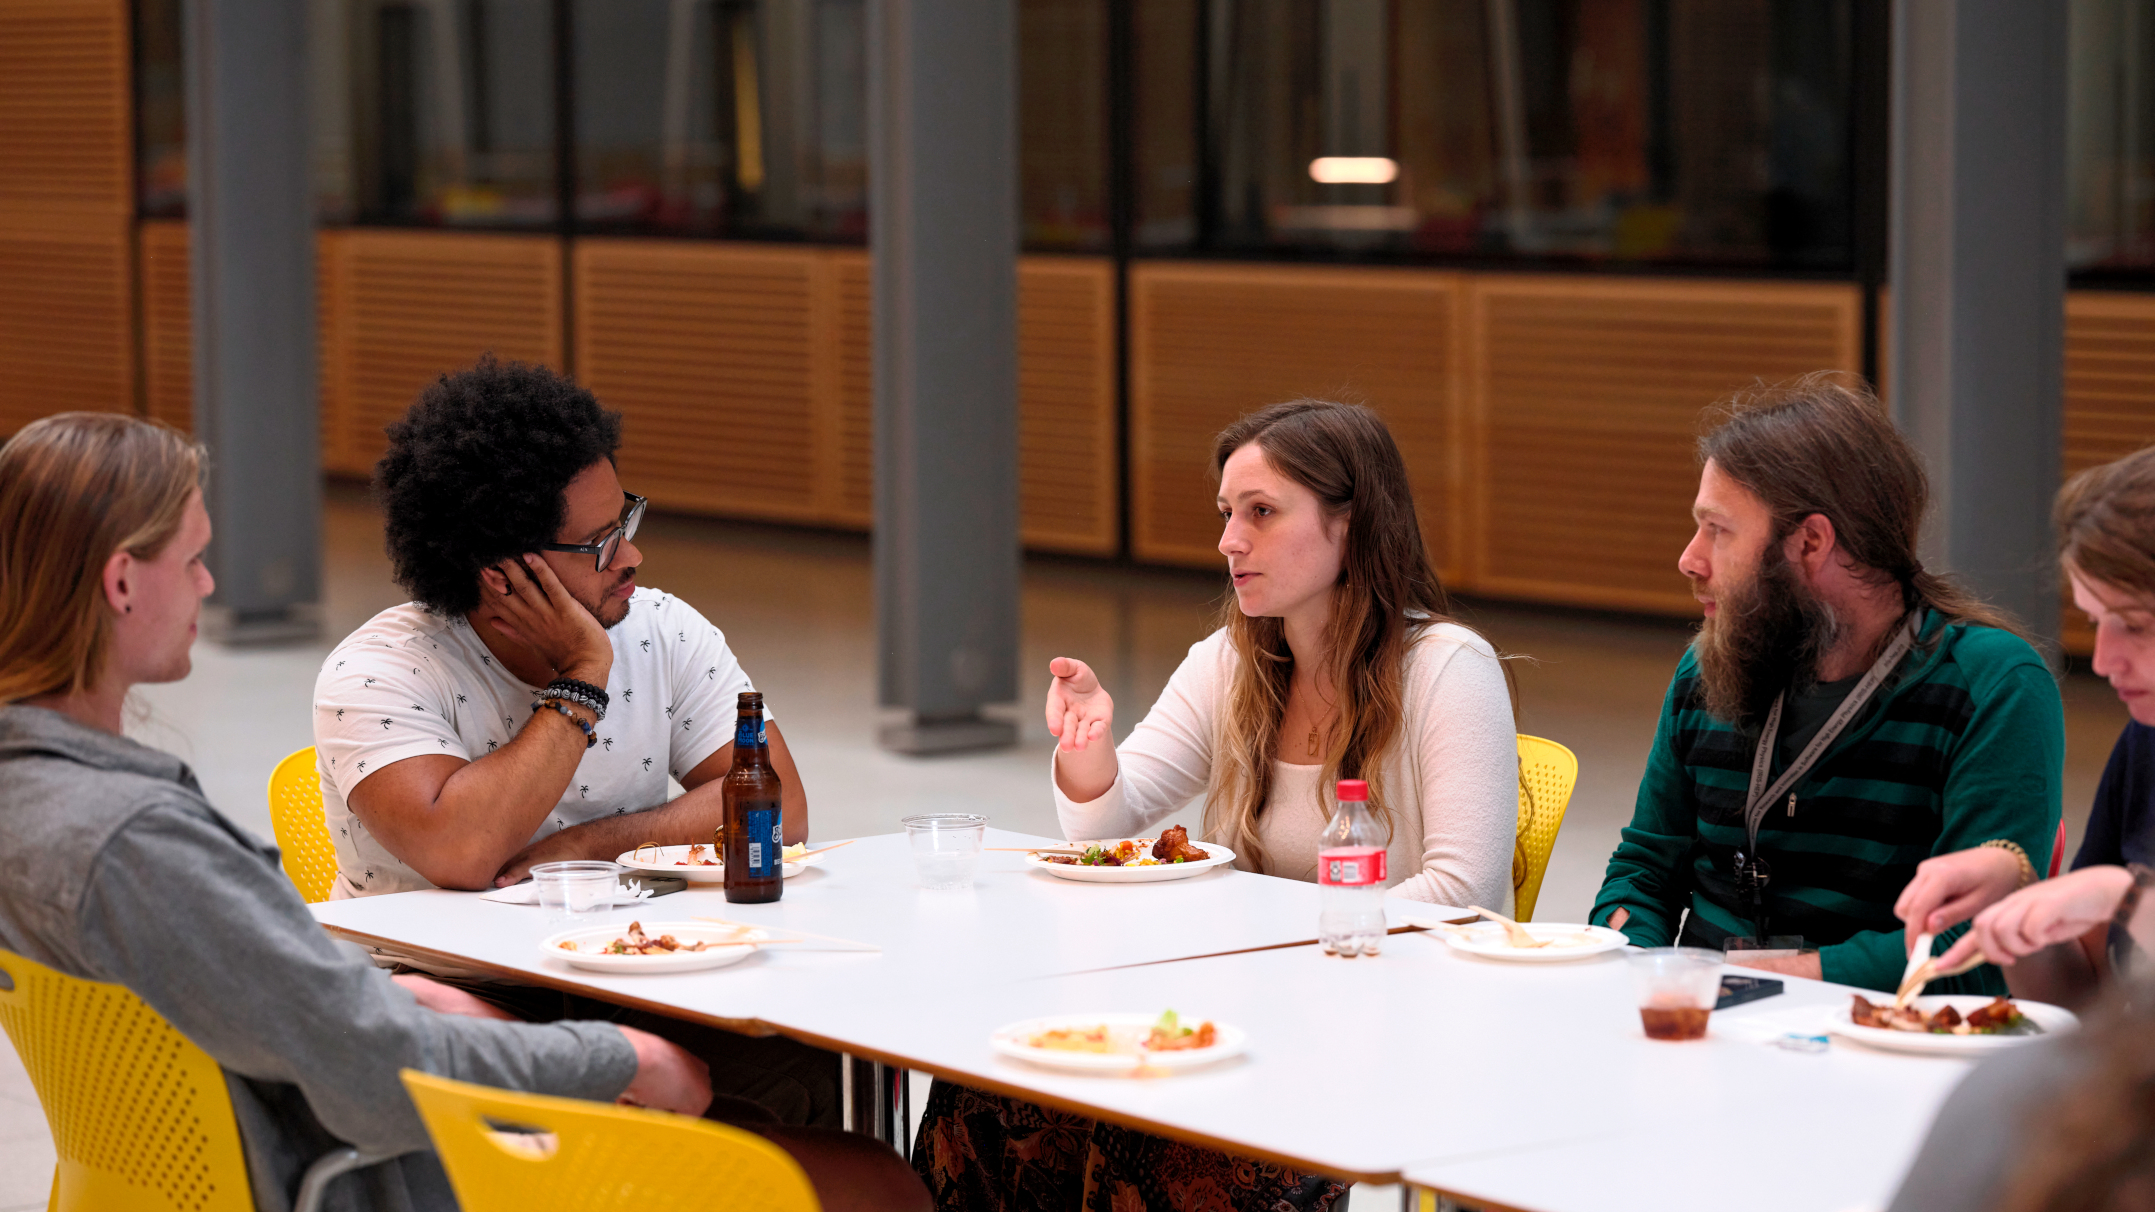
\includegraphics[width=\linewidth]{PHOTOS/DSCF2962.jpg}

%% \column{0.25\linewidth}
%% \includegraphics[width=\linewidth]{PHOTOS/DSCF3047.jpg}
\end{columns}

\begin{columns}
\column{0.33\linewidth}
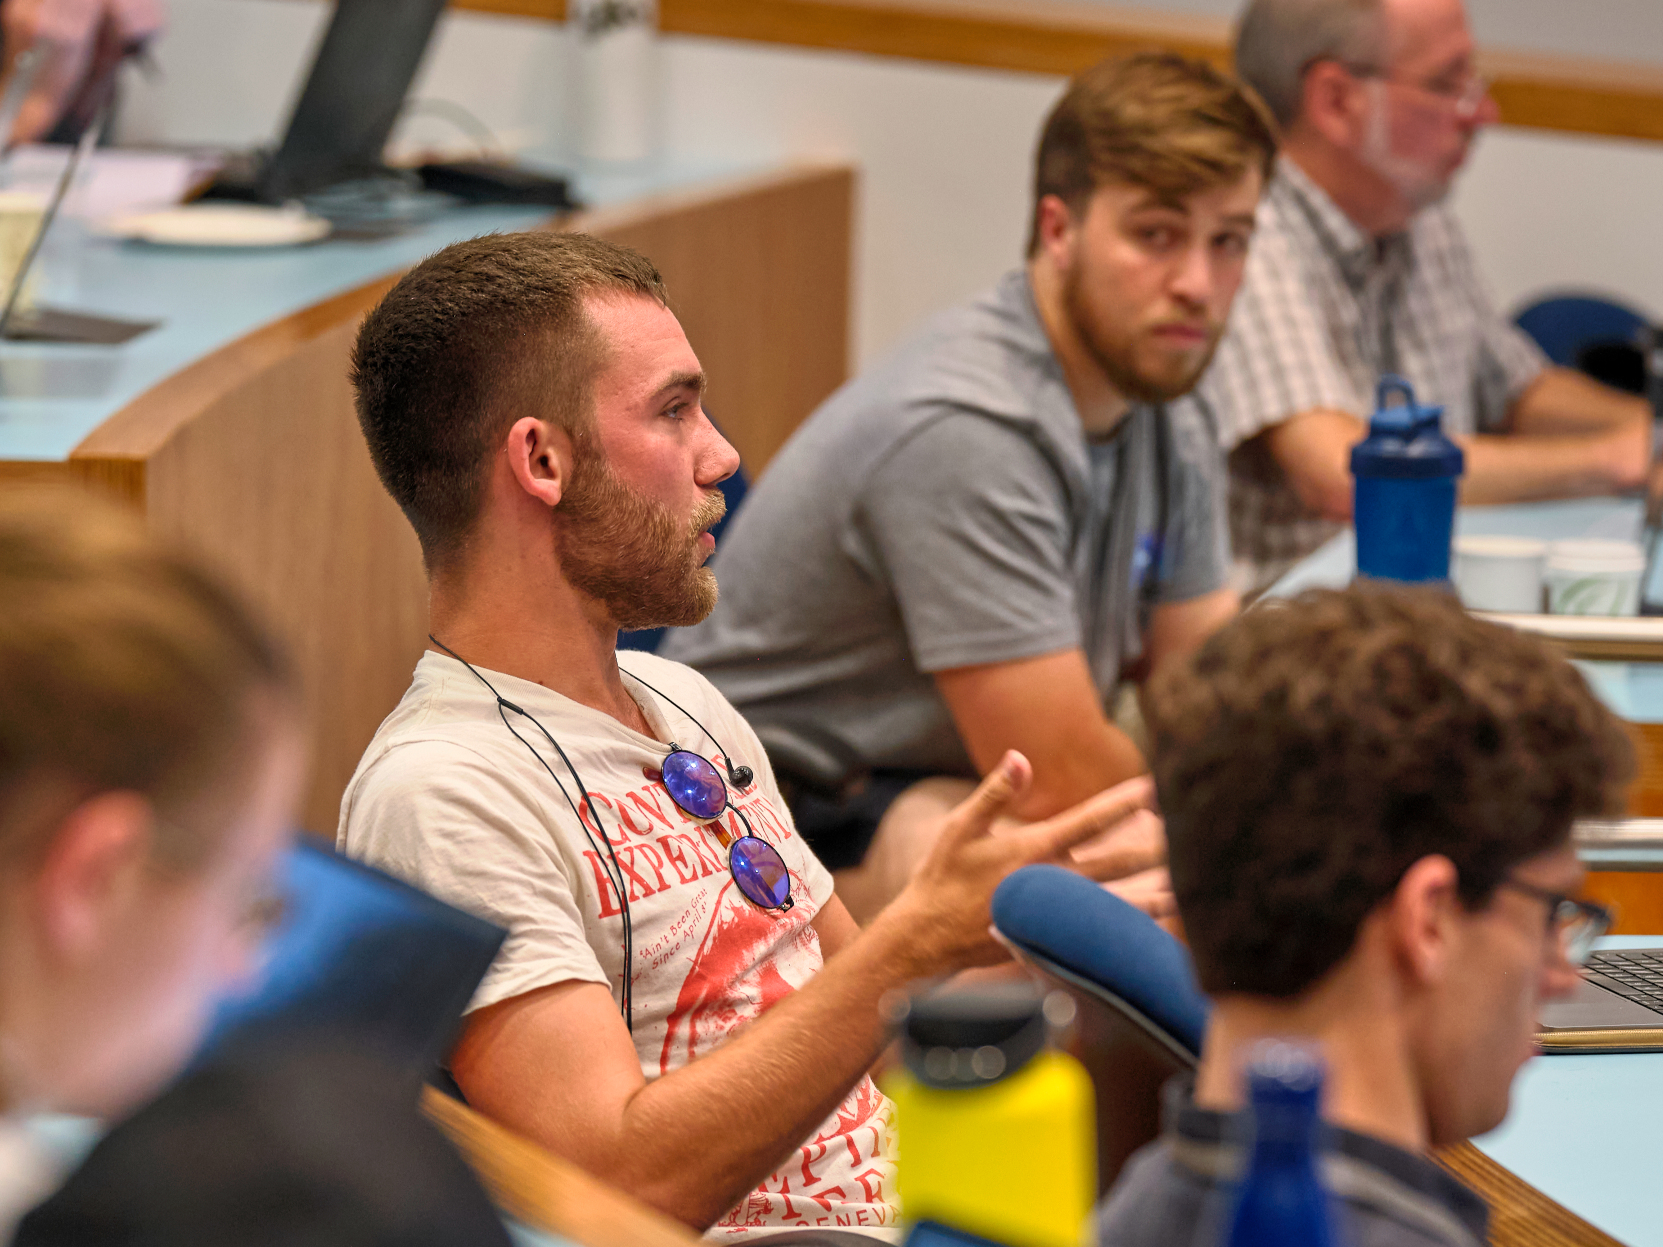
\includegraphics[width=\linewidth]{PHOTOS/DSCF2928.jpg}

\column{0.33\linewidth}
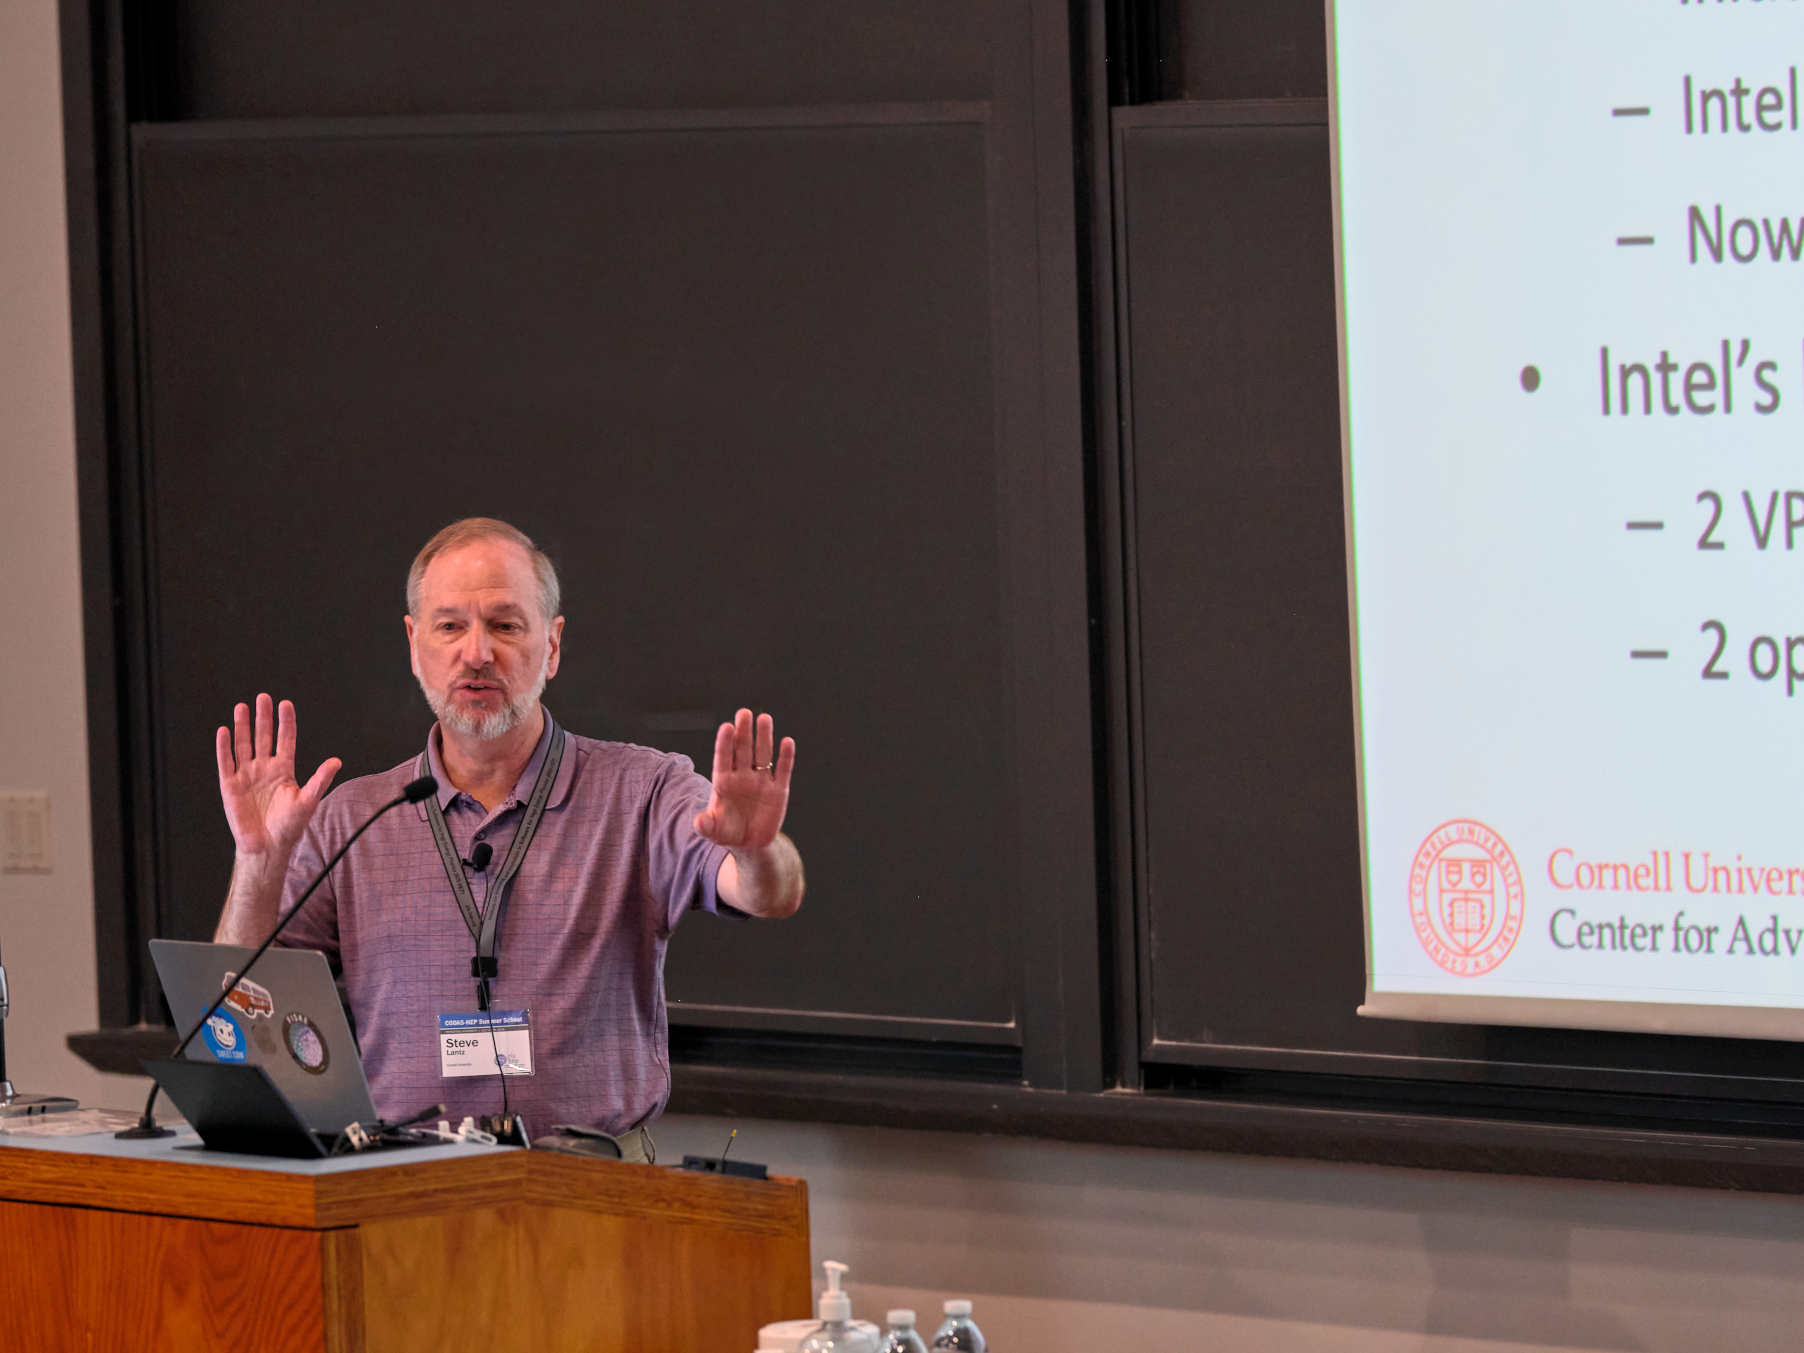
\includegraphics[width=\linewidth]{PHOTOS/DSCF2805.jpg}

\column{0.33\linewidth}
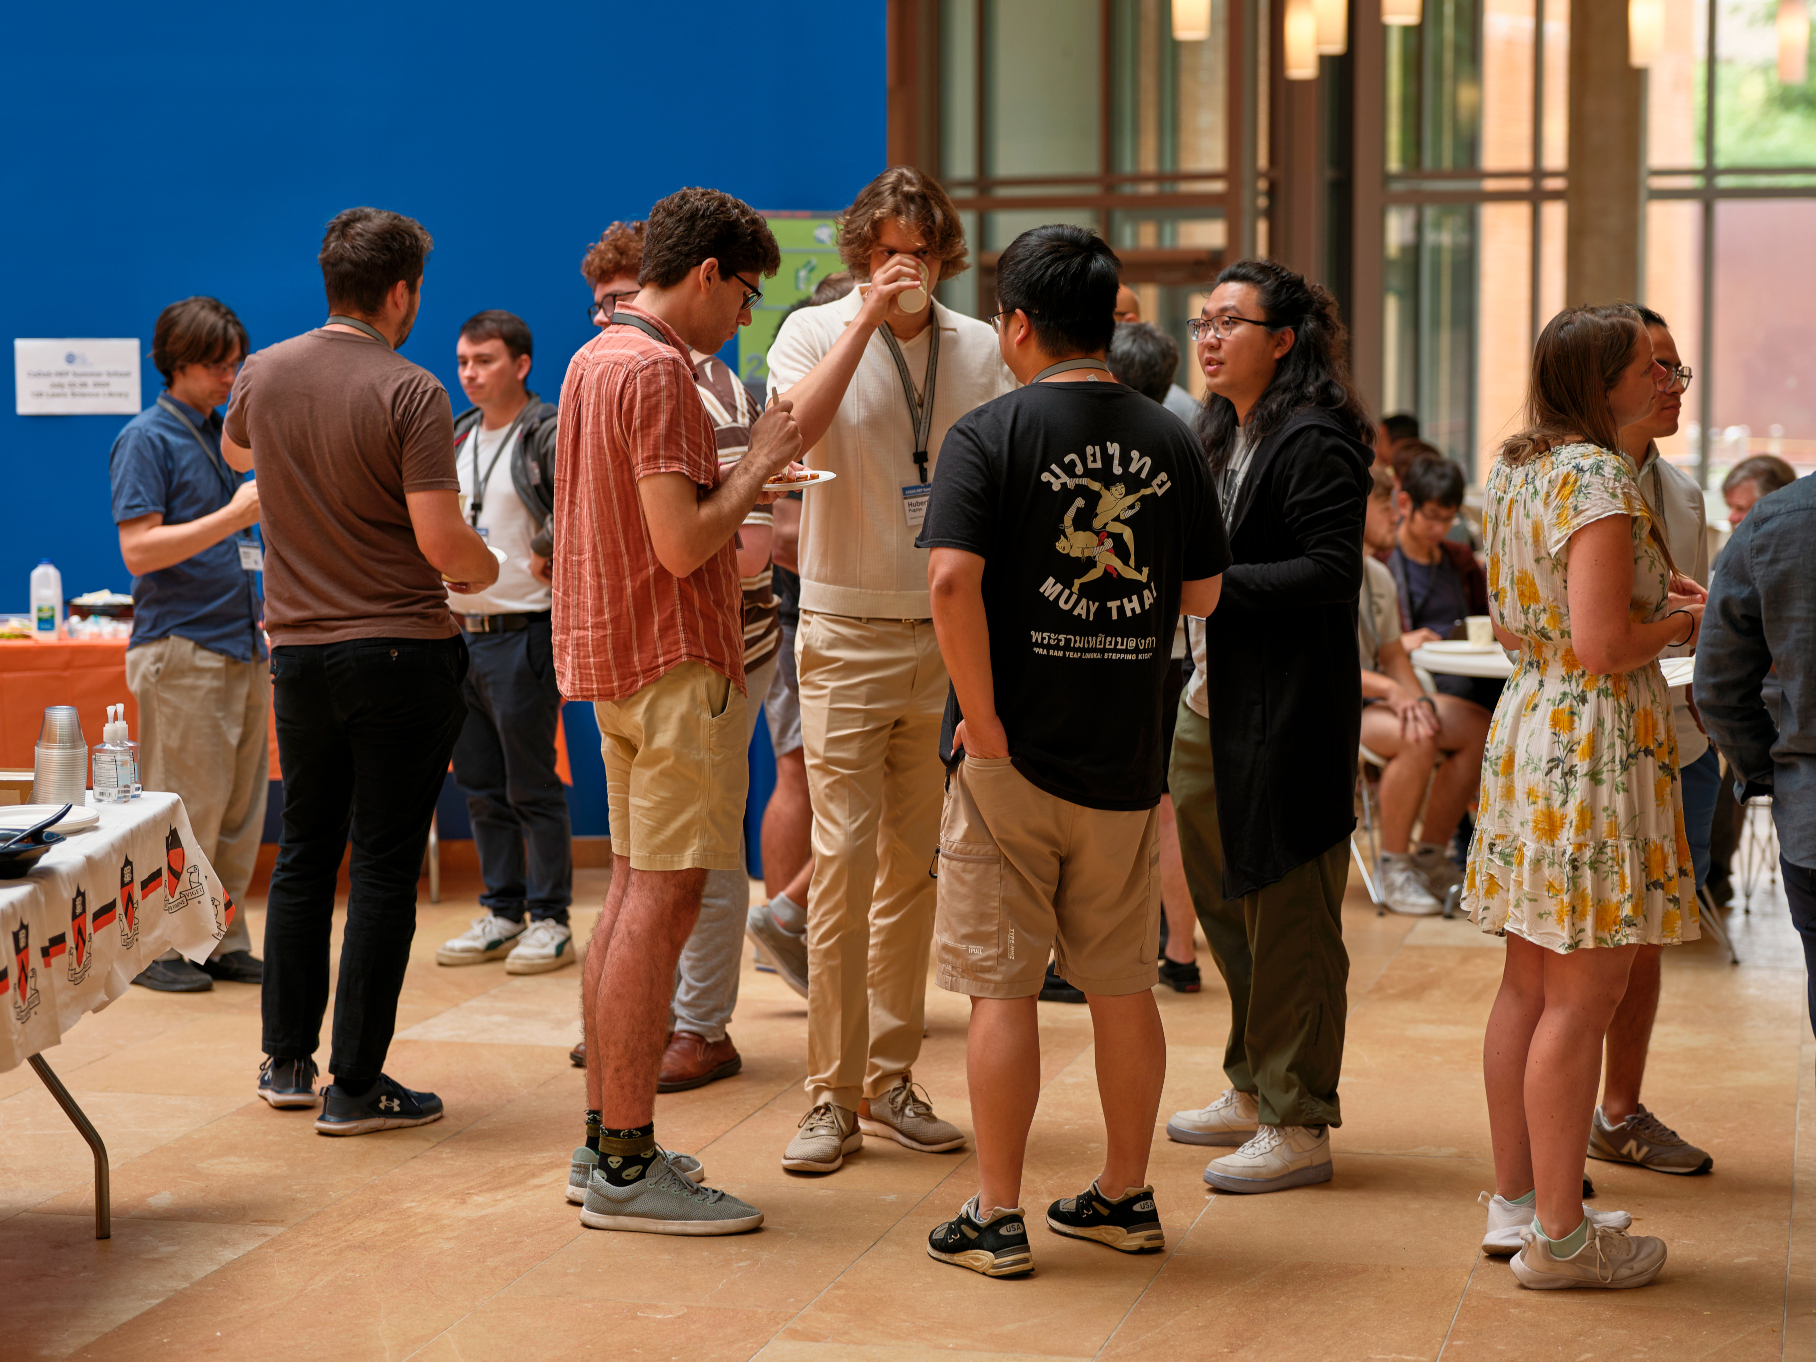
\includegraphics[width=\linewidth]{PHOTOS/DSCF2642.jpg}
\end{columns}
\end{frame}

\begin{frame}{All three events consisted of}
\Large
\vspace{0.5 cm}
\begin{itemize}\setlength{\itemsep}{0.25 cm}
\item<1-> Lecture-style presentations (PDF)
\item<2-> Lectures mixed with small problems (Jupyter)
\item<3-> Long exercises: 20 minutes through 2 hours
\item<4-> Catered breakfasts and lunches, coffee breaks
\item<5-> Social dinners and student bonding in dorms, pub crawls\ldots
\end{itemize}

\vspace{0.5 cm}
\large
\uncover<6->{Considerable sharing of teaching materials between events (including HSF-India), and from one year to the next.}

\vspace{0.25 cm}
\uncover<7->{With one exception, none of this material was from \textcolor{blue}{\url{hsf-training.org}}.}

\end{frame}

\end{document}
